% Chapter Template

\chapter{Working Environment Overview} % Main chapter title

\label{Chapter2} % Change X to a consecutive number; for referencing this chapter elsewhere, use \ref{ChapterX}

\lhead{Chapter 2. \emph{Working Environment Overview}} % Change X to a consecutive number; this is for the header on each page - perhaps a shortened title

%----------------------------------------------------------------------------------------
%	SECTION 1
%----------------------------------------------------------------------------------------

\section{UCL Internet Infrastructure}
The Catholic University of Louvain (UCL) is one of the biggest universities in Belgium. It gathers almost 30.000 students and about 10.000 other members from staff to teachers and researchers.\\

The university also owns several student campus. The headquarters of the UCL is located in the city of Louvain-la-Neuve. The campus gathering the health sciences is located in Woluwe-Saint-Lambert and more recently the cities of Tournai and Mons as well as Charleroi were added to the list.\\

Faced with such a scale, it is vital for the Catholic Univeristy of Louvain to develop a reliable and efficient Internet connection and wireless network able to deliver a connectivity throughout its campus and all users at all time.\\

The purpose the University enrolled in is to provide an Internet access and a connectivity according to the type of user who wants to connect. To do this, there are 3 main networks at the Catholic University of Louvain, each with a different SSID.\\

The univeristy also participates in the projet \texttt{eduroam} (which stands for education roaming). Eduroam is the secure, world-wide roaming access service developed for the international research and education community\cite{eduroam1}.\\

The eduroam system is a RADIUS-based infrastructure that uses the 802.1X security technology to allow for inter-institutional roaming. It allows the users visiting another institution connected to eduroam to log on to the WLAN using the same credentials the user would use if he were at his home institution\cite{eduroam2}.\\
The Catholic University of Louvain thus has a fourth network available with the SSID \texttt{eduroam} allowing the foreign students to be able to get an Internet connection at any time on the university locations.\\
The available networks at UCL are the following:
\begin{itemize}
	\item \texttt{student.UCLouvain}: Only for the students enrolled for the current year at UCL.
	\item \texttt{UCLouvain}: Only for university staff as well as for the researchers.
	\item \texttt{visiteurs.UCLouvain}: Accessible for guests invited by the university.
	\item \texttt{eduroam}: Education Roaming access.
\end{itemize}



\section{Hardware infrastructure}
Using the network monitoring software InterMapper\cite{intermapper} we see that the UCL network is composed of seven neighborhood routers (CtPythagore, CtHalles, CtLew, CtStevin, CtCarnoy, CtMichotte and CtSH1C). Six of them are present on the Louvain-la-Neuve campus and only CtLew is on the Wolluwé Campus. Those routers task is only routing.\\

Internet access is provided by Belnet via a 10GBit ethernet link directly connected to the CtPythagore. There is also a second 3GBit ethernet link connected to the CtHalles router but this link is never used. It is only a backup link in case of failure of the main one.\\

The infrastrucutre also has two main servers which are CtTier2 and CtAquarium. Those main servers are datacentres that contain the RADIUS servers as well as the LDAP servers.\\

Then for each building there is a switch and this switch is directly connected to one of the seven routers. Each of those switches has 48 ports that are connected to the access points inside the concerned building.\\
Concretely, in each building we find ethernet plugs that are connected to what we call concentration points. Those points contain commutators that is connected to the building switch that is connected to one of the main routers.\\
An important point to mention is that the network is not a full mesh.\\

Here is a simplified representation of the UCL network infrastructure:
\begin{figure}[H]
	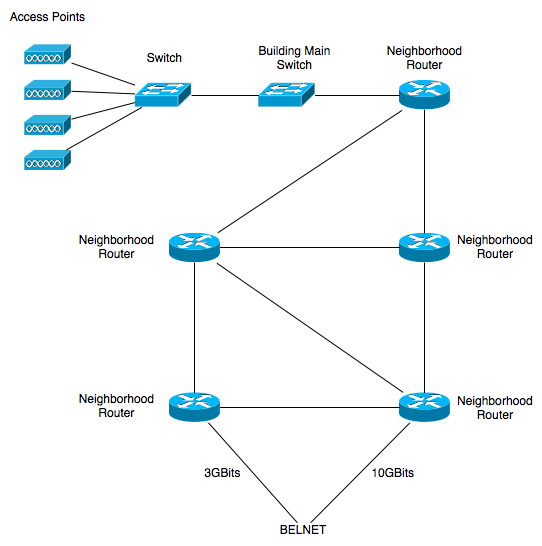
\includegraphics[width=.9\linewidth]{Pictures/Chapter2/infrastructure.png}
\end{figure}

\subsection{Network Topology}
Here is the representation of the network topology:
\begin{figure}[H]
	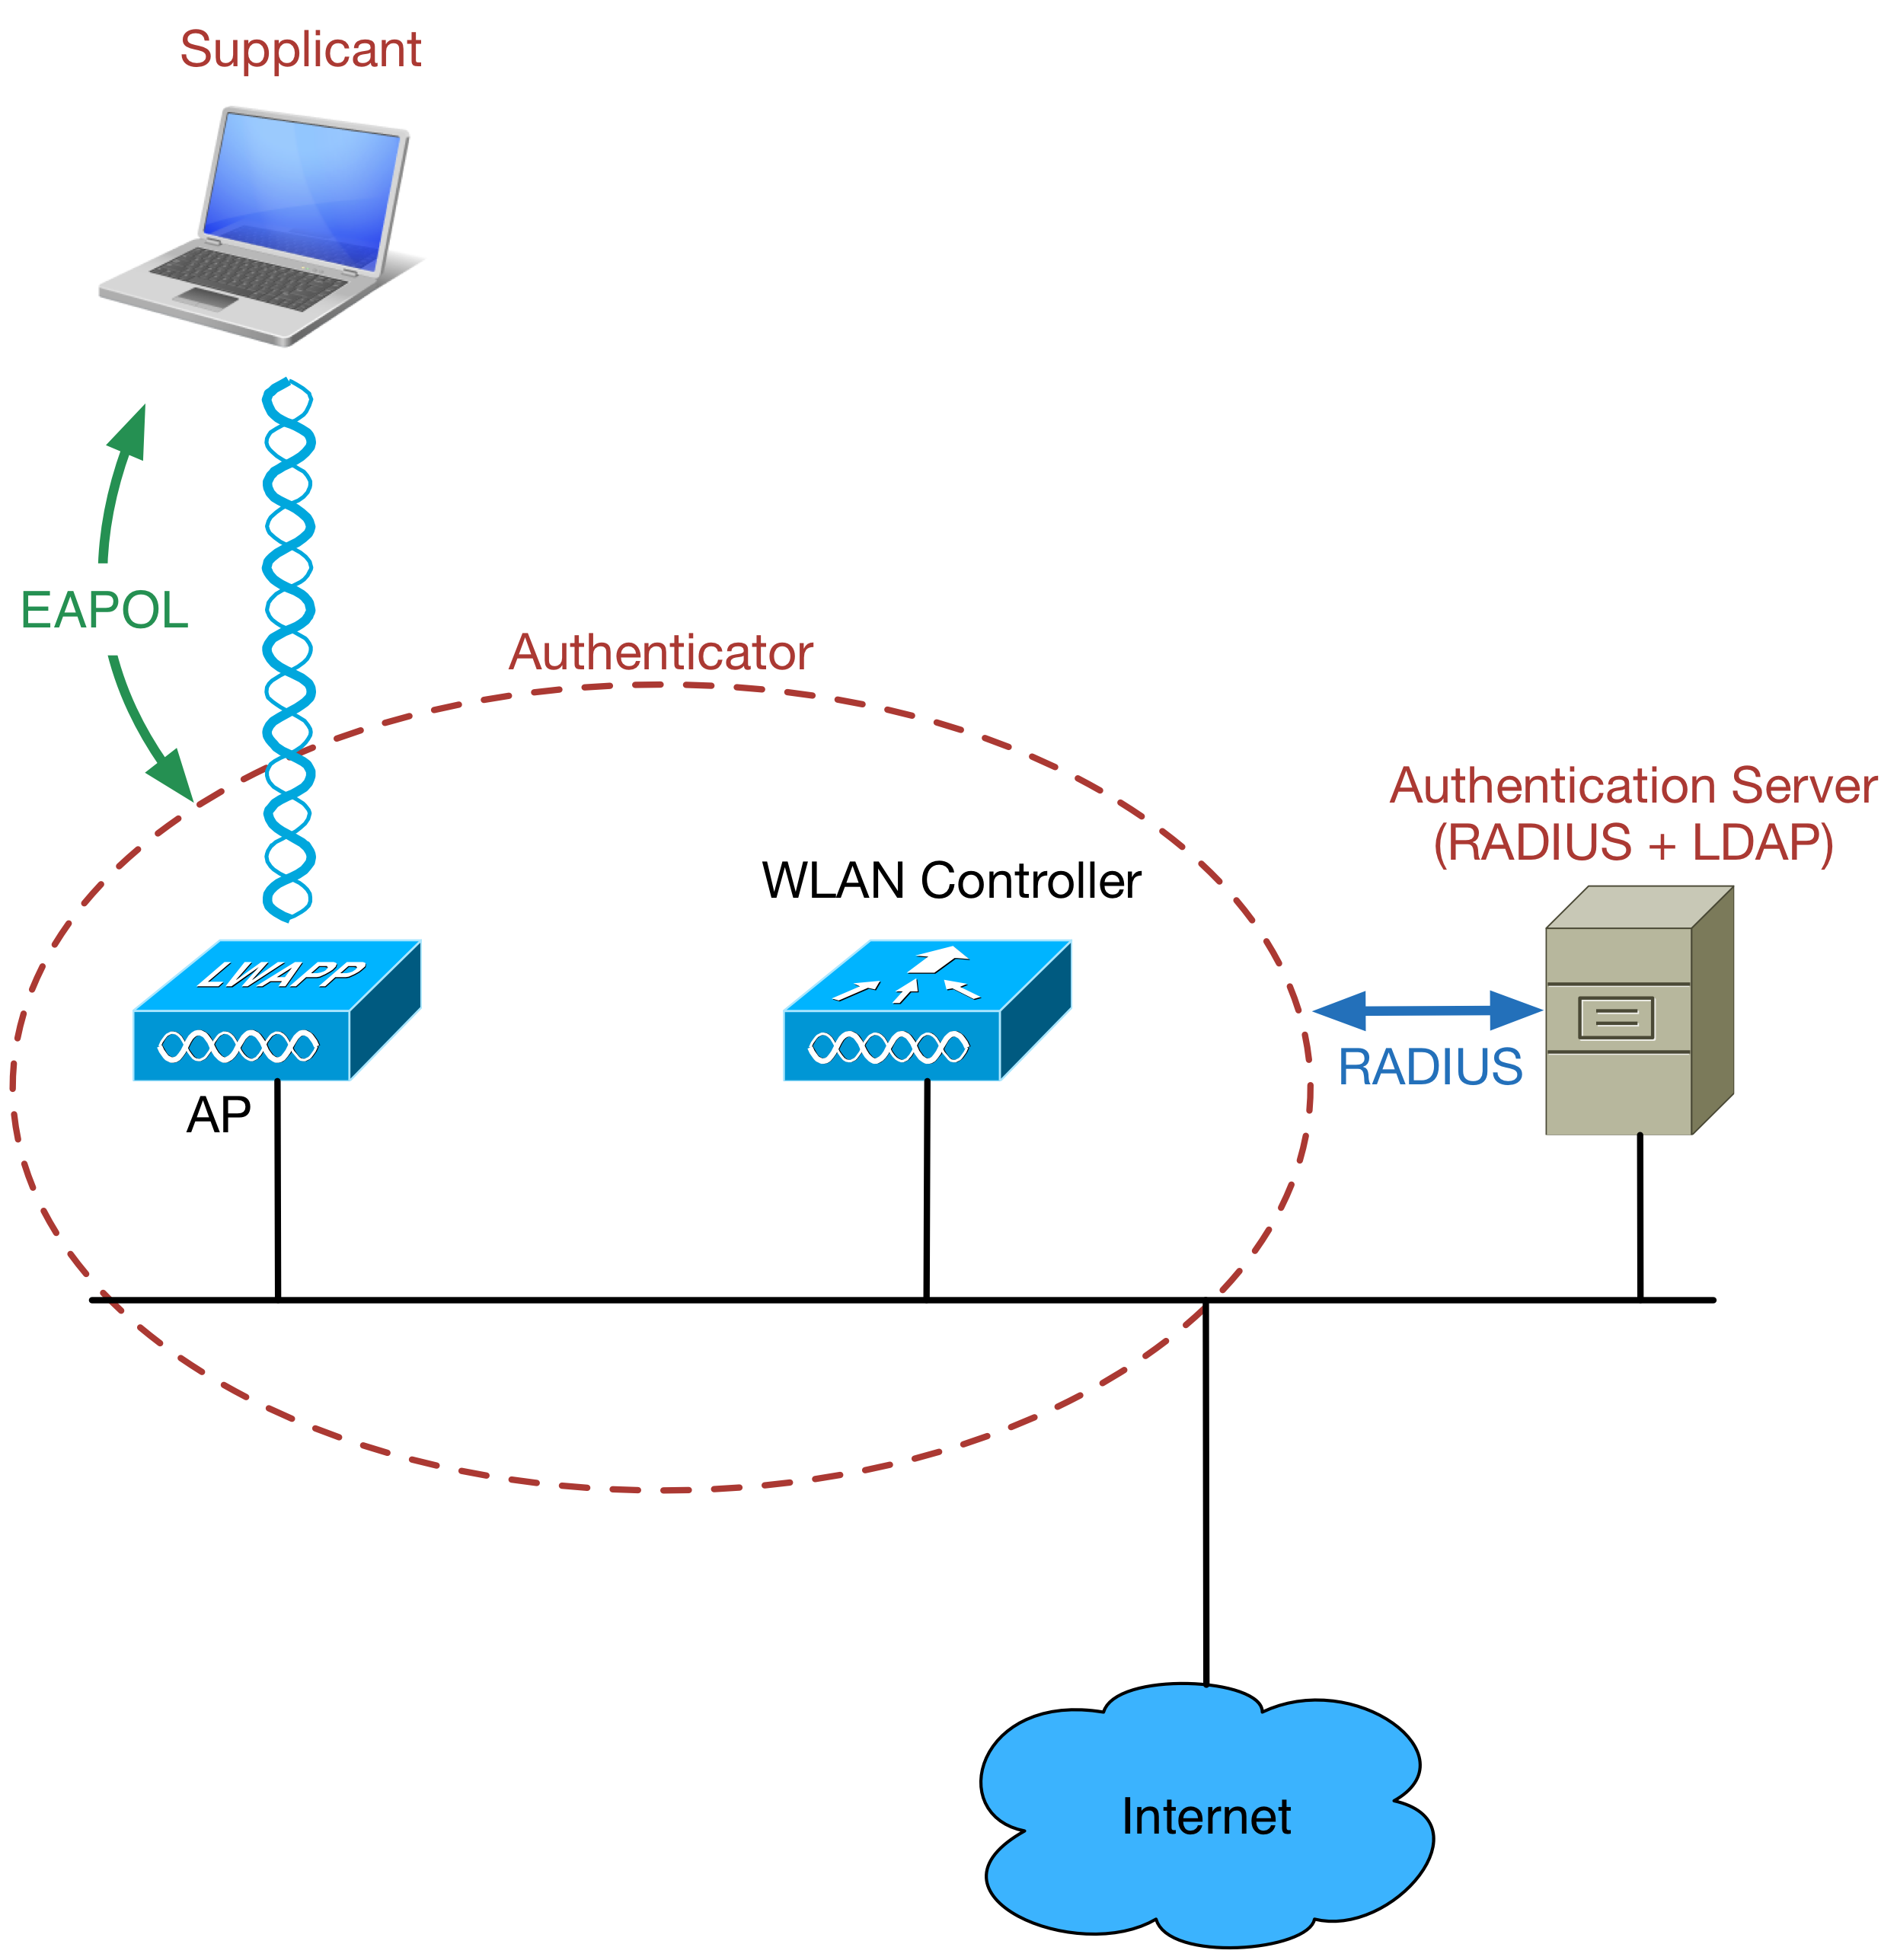
\includegraphics[width=.9\linewidth]{Pictures/Chapter2/topology.png}
\end{figure}
The Catholic University of Louvain has chosen to use the IEEE 802.1X protocol for user authentication. Thus when a user wants to connect to the WiFi, the access point will realize an EAP negociation with the supplicant. It transmits this EAP information to the controller who is going to interact with the RADIUS authentication server who, in turn, is going to asks information to the LDAP server. Once the RADIUS server authenticate the requesting user, the connection is established.




\section{Understanding the passive and active logs}